\begin{savequote}[75mm] 
And your heart hurts, mine does too\\
And it's just words and they cut deep
\qauthor{``Look What You've Done''- Drake} 
\end{savequote}

\chapter{Predicting Artist Influence with Siamese Networks}
Due to the limitations of the Document Influence Model, the need for richer feature representations and the scale of the audio dataset we collected, we next decided to investigate the application of deep learning, specifically an architecture known as a siamese convolutional neural network in modeling song-level influence. 

We address the following binary classification task: given as input a pair of two songs, what is the probability that there exists an influence relationship between the two artists who respectively recorded the songs?

\section{Model}
\subsection{Overview}
For the siamese network, we adopt a similar architecture as used by Koch et al. \cite{koch2015siamese} in predicting image similarity. Originally used for predicting similarity of two input images where the total number of image classes is large and the number of training instances for each class is sparse, siamese networks have been shown to be very successful in learning powerful descriptive features which generalize well to unseen pairs.

At a high level, our model takes in as input two mel-spectrogram representations of songs, which can essentially be viewed as ``images'' of the songs. Specifically, each mel-spectrogram is a two-dimensional array of floating point numbers with the first dimension corresponding to the frequency domain (128 total frequency bins in our case) and the second dimension corresponding to the number of timesteps in the time domain. Each of these inputs is fed separately through two copies of the same convolutional neural network (CNN). These two ``twin'' (hence the name siamese) CNNs extract a high-level fixed-length vector representation for each of the songs. The component-wise absolute distances between the extracted vectors for each of the songs are calculated, fed through a fully-connected perceptron layer, and then a sigmoid activation function is applied to output a probability between 0 and 1. A diagram of the model we used, including the input and output shapes for each layer, can be seen in the figure below:

\begin{figure}[H]
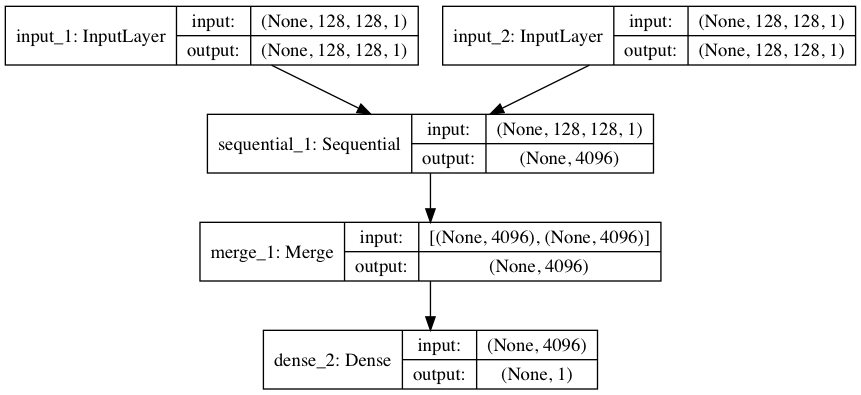
\includegraphics[width=\textwidth]{figures/siamese.png}
\caption{Diagram of siamese network architecture}
\end{figure}

\texttt{input\_1} and \texttt{input\_2} correspond to the 2 mel-spectrogram snippets of an input pair that we take in. A note on dimensions, taking the input dimensions of \texttt{input\_1}, $(None, 128,128,1)$ as an example: The first dimension corresponds to batch size, which was left as $None$ in the diagram for the sake of generality. The second and third dimensions correspond to the fact that each mel-spectrogram snippet used is a 128x128 matrix of real-valued numbers. The fourth dimension corresponds to the number of channels in the image, which was simply $1$ in our case (in color image applications for instance, channel size is commonly set to $3$ to deal with the RGB channels separately).

Each of the inputs are separately fed into the same CNN, called \texttt{sequential\_1} in our diagram for feature extraction. Shortly, we will discuss this CNN in further detail.

\texttt{sequential\_1} extracts a fixed-length vector representation of each song. In \texttt{merge\_1} the absolute element-wise differences between the vector representations for each song are calculated, and then in \texttt{dense\_2} the output is passed through one last fully connected layer with learnable weights, and a sigmoid activation function is applied.

The parameters for each of the layers of our siamese network are trained using the standard backpropagation algorithm against the standard binary cross-entropy loss function.

We implemented the model using the Keras library\cite{chollet2015keras} in Python.

\subsection{CNN Architecture}
We now give a more detailed description of the CNN architecture we used (\texttt{sequential\_1} in the figure above), depicted in detail in the figure below:

\begin{figure}[H]
\centering
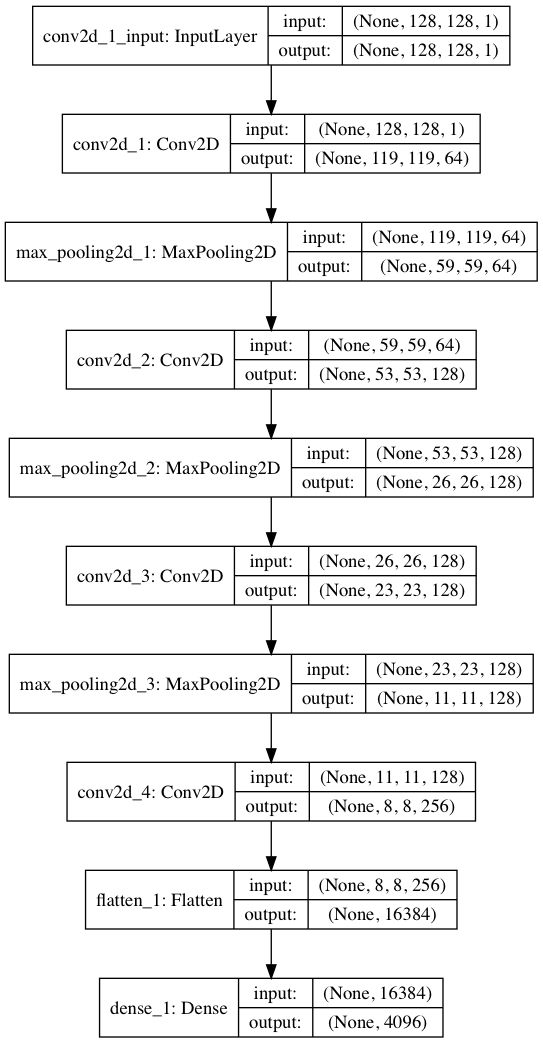
\includegraphics[width=8cm]{figures/conv_net.png}
\caption{Diagram of CNN architecture}
\end{figure}

Our CNN architecture consists of 4 convolutional layers with the ReLU activation function, alternated with 3 max pooling layers. The first convolutional layer consists of 64 10x10 convolutional filters, the second convolutional layer consists of 128 7x7 filters, the third convolutional layer consists of 128 4x4 filters, and the fourth convolutional layer consists of 256 4x4 filters. Max pooling is performed in between convolutional layers in order to downsample the image. Finally the results from the last convolutional layer are flattened and passed through a fully-connected layer with the sigmoid activation function before being passed to \texttt{merge\_1} for calculation of distance between the feature vector representations for each song.



\section{Experimental Setup}

\subsection{Sampling of Songs}
Due to RAM limitations with the GPU we had access to for training and the need for reasonable training time, we were not able to use the entire mel-spectrogram representation corresponding to the full 30 seconds of audio we had access to for each song. Instead during training we randomly sampled contiguous 3 second samples on the fly from the full mel-spectrogram during each epoch (thereby generating different 3 second samples for each particular song each new epoch). Though using the full mel-spectrogram would have preserved the most information, given that previously \cite{van2013deep} 3 second samples have been used in other music audio tasks involving deep learning and our eventual results, this was likely a reasonable simplification.

In addition to sampling at the song-level, to further simplify training time, we only used the audio from one song for each artist. 

\subsection{Train-Validation Split}
As with any binary classification task, balance between the positive and negative example classes was a concern. In this case, our positive examples were derived from the ground truth AllMusic influence graph. Specifically, out of all edges in the ground truth graph, we had audio corresponding to 88,853 of them, and we used these pairs as our positive examples. We artificially generated negative examples of pairs where influence does not exist by randomly sampling for 88,853 artist pairs that do not correspond to edges in the ground truth graph, thereby creating a balanced number of positive and negative pairs overall. These combined 177,706 pairs were then randomly split into 80\% training and 20\% validation data. 

\subsection{Training}
Training was performed on a Tesla K20Xm GPU on Harvard's Odyssey cluster. We used a batch size of 16 and the Adam optimizer \cite{kingma2014adam} (an adaptive variant of standard Stochastic Gradient Descent), with training concluding after validation loss stopped decreasing for 5 epochs. In total, training took 51 epochs. 

\section{Results}
The loss and accuracy curves on both the training and validation sets can be seen in the figures below:

\begin{figure}[H]
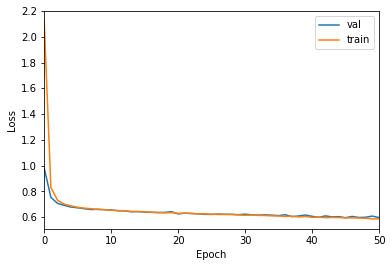
\includegraphics[width=\textwidth]{figures/loss.png}
\caption{Plot of training loss curves for siamese network}
\end{figure}

\begin{figure}[H]
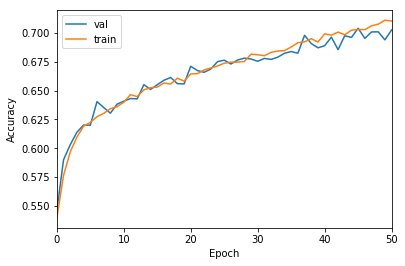
\includegraphics[width=\textwidth]{figures/accuracy.png}
\caption{Plot of training accuracy curves for siamese network}
\end{figure}

On the validation set, the final model had an accuracy of $0.7005$. For comparison, due to the balanced nature of our dataset, a completely random model (using the result of a fair coin flip to guess whether an influence relationship exists or not between two input songs) would have had an accuracy of approximately $0.5$. Other metrics for the final model are summarized in the table below:

\begin{table}[H]
\centering
\caption{Accuracy metrics for trained siamese network on validation set}
\label{my-label}
\begin{tabular}{|l|l|}
\hline
Metric    & Value  \\ \hline
Accuracy  & 0.7005 \\ \hline
Precision & 0.6875 \\ \hline
Recall    & 0.7353 \\ \hline
F1 Score  & 0.7106 \\ \hline
\end{tabular}
\end{table}


\subsection{Same-Song Sample Prediction}
As a sanity check, we also tested the model's accuracy by creating pairs of samples where both samples were from the same song. Despite not being trained on this task, the model had an accuracy of $0.9018$ for identifying that the samples were from the same song.

\subsection{Intergenre vs. Intragenre Prediction}
We evaluated accuracy, precision and recall for intergenre v. intragenre prediction, using artist genre metadata information we gathered from AllMusic. Intergenre is defined as the two songs in the pair coming from artists of different genres (i.e. Jazz v. Classical) and intragenre is defined as sharing the same genre. The results are summarized in the table below:

\begin{table}[H]
\centering
\caption{Accuracy metrics for intergenre vs. intragenre prediction}
\label{my-label}
\begin{tabular}{|l|l|l|}
\hline
Metric    & Same Genre & Different Genre \\ \hline
Accuracy  & 0.7134     & 0.6971          \\ \hline
Precision & 0.8484     & 0.4198          \\ \hline
Recall    & 0.7676     & 0.6471          \\ \hline
F1 Score  & 0.8060     & 0.5092          \\ \hline
\end{tabular}
\end{table}

We see that across all metrics, the model outperforms on prediction when both artists are from the same genre vs. when the two artists are from different genres. In particular, we see that precision greatly suffers when the artists are from different genres.

\subsection{Average Prediction Accuracy by Time Between Release Years of Songs}
We also evaluated the average accuracy of our siamese network vs. the number of years between the release years of songs in input pairs:

\begin{figure}[H]
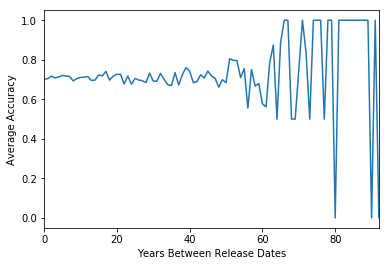
\includegraphics[width=\textwidth]{figures/acc_by_year.png}
\caption{Plot of average accuracy vs. time between release years of songs}
\end{figure}

Note that the wide variance in the right-hand portion of the plot is due to the small number of samples that had a year difference greater than $60$, especially when it came to positive examples of influence relationships. To test for a relationship between time between release years and model accuracy, we conducted a likelihood-ratio test (LRT) of a logistic regression model including time as a single predictor vs. a null intercept-only model, with a binary indicator for whether the siamese network was accurate as the response variable for both models. The LRT returned $p=0.77$, so we failed to reject the null model and concluded that there was no statistically significant relationship between time between release years and model accuracy.

\subsection{Qualitative Error Analysis}
To get a better sense of how our siamese network was making errors (i.e. predicting influence relationships when there existed none), we filtered out for cases where the model predicted with very high probability ($>0.95$) that there existed an influence relationship when there in fact was none. These cases, which we will refer to as \textit{high probability errors} are outlined in the table below, with the respective members of the pair separated by a comma and each member written in the format ``Artist Name - Song Name'':

\begin{table}[H]
\centering
\caption{Examples of high probability errors for siamese network}
\begin{tabular}{lr}
\hline
 Input Pair                                                             &   Predicted Probability \\
\hline
 Brainiac - Hot Seat Can't Sit Down, Nirvana - Been a Son               &                0.985368 \\
 Buzzcocks - Fast Cars, Xasthur - Trauma Will Always Linger             &                0.976721 \\
 Babyland - Past Lives, Ramones - Gimme Gimme Shock Treatment           &                0.976054 \\
 Tony Iommi - Paranoid, Iron Maiden - Powerslave                        &                0.973814 \\
 Nine Inch Nails - The Hand That Feeds, Badlands - Ride the Jack        &                0.973143 \\
 Winter - Winter, Neil Young - The Needle and the Damage Done           &                0.972291 \\
 Fatboy Slim - Right Here Right Now, Swans - I Am the Sun               &                0.970423 \\
 Jimi Hendrix - Machine Gun, Roger Miller - Old Friends                 &                0.96569  \\
 Nirvana - Been a Son, Gorilla Biscuits - New Direction                 &                0.96561  \\
 Ramones - Gimme Gimme Shock Treatment, Yves Deruyter - The Rebel       &                0.961905 \\
 Bo Diddley - Road Runner, Zaiko Langa Langa - Egide                    &                0.960632 \\
 Leila Pinheiro - Renata Maria, Fatboy Slim - Right Here Right Now      &                0.960359 \\
 Corrosion of Conformity - Stare Too Long, KT Tunstall - Suddenly I See &                0.95792  \\
 Skywave - Here She Comes, NOFX - Bob                                   &                0.951591 \\
 Hawkins Family - Changed, Lee "Scratch" Perry - Heavy Voodoo           &                0.95039  \\
\hline
\end{tabular}
\end{table}

In the vast majority of these cases, both members of the input pair belong to the same genre of Pop/Rock, so this may partially explain why the model has difficulty, though in section 5.3.2 we did note that the model tends to perform better on intragenre prediction on aggregate, so this is not in line with that trend.

Listening to the audio samples themselves, the mistakes the model made seem reasonable for the most part. For instance, the two tracks in the first pairing --- Brainiac - Hot Seat Can't Sit Down, Nirvana - Been a Son --- do overlap acoustically. Both tracks feature male lead vocals with similar timbres, grungy guitar and a strong rock backbeat. In fact, given the proximity of the active years for the two bands (1992-1997 for Braniac and 1987-1994 for Nirvana), it is possible that one of the bands influenced the other even if that is not reflected in the AllMusic influence graph.

On the other hand, the pairing of Bo Diddley - Road Runner, Zaiko Langa Langa - Egide, which the siamese network predicts to be an example of an influence relationship with probability 0.95 appears rather out-of-place when listening to the two tracks alongside one another. The former is a 1960s 12-bar blues by an American musician while the latter is an upbeat-sounding 1995 dance number by a group from the Democratic Republic of the Congo. The closest sonic element that the two tracks appear to have in common is a similar tempo, but that is about it.

While we will not exhaustively go through each of these pairings, this sort of qualitative analysis does suggest elements that the network may be picking up on, such as timbre, groove, instrumentation and tempo, which are indeed some elements that a human listener would pay attention to as well. That said, this is to a certain extent speculative; the convolutional filters of the network could just as well be latching onto some other aspect of the mel-spectrogram representation not discussed here. Though there have certainly been recent developments in interpreting CNNs \cite{olah2018the}, at the moment there is simply no way to tell for certain what specific elements of the songs our model focuses on in generating predictions.

\newpage
\section{Model Application: Ranking Influence}
One natural influence-related question one may ask is, given a collection of an artist's influencers (people who influenced the artist in question), how might we rank the relative importance of these influencers in terms of impact on that artist's music? Indeed, this question is particularly interesting in the case of the ground truth influence graph from AllMusic given that it only contains edges indicating influence relationships with no information about the relative \textit{strength} of these relationships.

\subsection{Ranking Algorithm Definition}
We propose the following algorithm which applies our trained siamese network to answer the question of the relative ranking of influencers:

\begin{enumerate}
    \item For a given artist $u$, get the set $A_u$ of all influencers (ancestors) of $u$ according to the ground truth graph. Therefore $\{(a, u) : a \in A_u\}$ would be the set of all directed edges terminating at node $u$ in the ground truth graph. 
    \item Estimate the average probability of influence for an influencer-artist pair $(a, u)$: create an input pair for the trained siamese network by randomly sampling a 3-second snippet of the respective mel-spectograms for each artist in the pairing and run the trained model to obtain a predicted probability of influence $p_1^a$ where the superscript indicates the influencer we are considering and the subscript indicates which sample we are on. 
    Independently sample a total of $n$ times for this influencer-artist pair, so we have $n$ influence probabilities $p_1^a, p_2^a ... p_n^a$. Take the mean to get an estimated average probability of influence for the influencer-artist pair $\hat{p^a} = \dfrac{\sum_{i=1}^n p_i^a}{n}$.
    \item Repeat step (2) for all $a \in A_u$ to get an estimated average probability of influence for every influencer-artist pair.
    \item Normalize the estimated average probabilities of influence for each influencer-artist pair to yield an \textit{estimated influence proportion} for each influencer: $\hat{p}_{norm}^a = \dfrac{\hat{p}^a}{\sum_{a' \in A_u}{\hat{p}^{a'}}}$
\end{enumerate}

Therefore in the end we obtain an estimated influence proportion for each influencer-artist pair $\hat{p}_{norm}^a$ with $\sum_{a \in A} \hat{p}_{norm}^a = 1$. A higher value of $\hat{p}_{norm}^a$ for a given influencer can be interpreted as the influencer being more influential on the artist $u$, and we consequently now have a method of ranking influencers.


\subsection{Qualitative Analysis}
To see this algorithm in action, we apply it to rank the influencers of J. Cole, a popular Rap artist and Charlie Parker, widely regarded as the greatest jazz alto saxophonist of the 20th century, using $n=100$ (100 three second samples per each influencer-artist pairing). The rankings of the influencers in decreasing order of estimated influence proportion for both of these artists as determined by our algorithm can be seen in the tables below, accompanied by qualitative analyses from a musicological perspective:

\begin{table}[H]
\centering
\caption{Influence proportions of J. Cole's influencers by our ranking algorithm}
\begin{tabular}{lr}
\hline
 Influencer Name   &   Estimated Influence Proportion \\
\hline
 2Pac              &                        0.124236  \\
 Pharrell Williams &                        0.124146  \\
 Jay-Z             &                        0.124084  \\
 Nas               &                        0.122706  \\
 Clipse            &                        0.116895  \\
 OutKast           &                        0.108001  \\
 Eric B. \& Rakim   &                        0.101246  \\
 Pete Rock         &                        0.0903422 \\
 Murs              &                        0.0883447 \\
\hline
\end{tabular}
\end{table}

\textbf{Analysis}: According to J. Cole himself, his favorite rappers as a child were 2Pac and Jay-Z \footnote{\url{http://www.musictimes.com/articles/11093/20140930/j-cole-talks-jay-z-tupacs-influence-career-watch.htm}}, who appear as the number 1 and number 3 influencers respectively for him according to our ranking algorithm. In another interview, J. Cole stated that in order, his favorite rappers of all time were: 2Pac, Biggie, Nas, Jay-Z, and Andre 3000 (one-half of the group OutKast) \footnote{\url{https://www.hotnewhiphop.com/j-cole-lists-top-5-rappers-recalls-worshipping-eminem-news.13210.html}}. Discounting the artists in this listing who do not appear in the graph we scraped from AllMusic, the relative ordering given personally by J. Cole of 2Pac, Nas, Jay-Z and OutKast corresponds very closely to the ordering given by our algorithm in the table above. Recalling the discussion of various definitions of influence posed in the introduction, it is perhaps important to note that in real life Jay-Z was J. Cole's first mentor and in fact Jay-Z's label was the first one J. Cole signed to. Given the close personal relationship between the two, it is therefore perhaps plausible that Jay-Z has had a slightly greater impact than Nas on J. Cole's music as well, which is what our algorithm would appear to suggest.

\begin{table}[H]
\centering
\caption{Influence proportions of Charlie Parker's influencers by our ranking algorithm}
\begin{tabular}{lr}
\hline
 Influencer Name   &   Estimated Influence Proportion \\
\hline
 Roy Eldridge      &                        0.0669437 \\
 Louis Armstrong   &                        0.0664712 \\
 Ben Webster       &                        0.0659504 \\
 Coleman Hawkins   &                        0.0641175 \\
 Benny Carter      &                        0.0634215 \\
 Barney Kessel     &                        0.0631203 \\
 Buster Smith      &                        0.0627861 \\
 Lester Young      &                        0.0623917 \\
 Art Tatum         &                        0.0620452 \\
 Erskine Hawkins   &                        0.0619891 \\
 Johnny Hodges     &                        0.0617768 \\
 Don Byas          &                        0.0614892 \\
 Illinois Jacquet  &                        0.0609022 \\
 Count Basie       &                        0.0594951 \\
 Jay McShann       &                        0.059046  \\
 Jimmy Dorsey      &                        0.058054  \\
\hline
\end{tabular}
\end{table}

\textbf{Analysis}: At first glance, this ranking appears puzzling because the top 2 artists, Roy Eldrige and Louis Armstrong are trumpet players whereas Charlie Parker is a saxophone player. This seems strange since in jazz, usually (though not always) an artist's strongest influencers tend to be players of the same instrument. However, listening to the audio clip of Charlie Parker used for sampling reveals a plausible explanation: the audio clip is of the standard ``A Night in Tunisia'', which features the trumpeter Dizzy Gillespie playing the song's melody alongside Parker. According to AllMusic, Gillespie himself was influenced by Eldrige and Armstrong. Thus the first two entries of our ranking make more sense given that our trained siamese network has no mechanism by which we can dictate which instrument to focus on, and furthermore this suggests that our model is able to pick up on instrument-specific timbres such as trumpet. Looking further down the ranking from our algorithm, Lester Young and Buster Smith should perhaps rank higher given that they are mentioned by critics as clear influencers of Charlie Parker \footnote{\url{https://www.allmusic.com/artist/charlie-parker-mn0000211758/biography}}, though they do both appear in the upper half of the ranking.

Our proposed algorithm for ranking influence is still preliminary and requires further validation. Though the suggested trends as discussed above for the two examples of J. Cole and Charlie Parker are interesting, they obviously are not definitive proof of the efficacy of the algorithm. One potential cause for concern for instance is that the estimated influence proportions tend to be fairly close to one another in magnitude. That said, as an application of our trained model, the algorithm does demonstrate the versatility of our approach to modeling musical influence through siamese networks.

\section{Discussion}
\subsection{Comparison to Morton and Kim}
Morton and Kim \cite{morton2015acoustic} used deep belief networks \cite{hinton2006fast} as feature extractors from spectral representations of songs before using logistic regression for classification. They treated influence prediction as a multi-label classification problem with 10 total classes, using the top 10 most influential artists from AllMusic in terms of outdegree as the classes. They achieved an F1-Score of approximately 0.4, though it is important to note that their results cannot directly be compared with ours due to differences in problem setup.

In contrast, our system using siamese convolutional neural networks is arguably more general. Instead of having a fixed number of artists as possible labels, our model takes in as input a pair of samples of songs and returns a binary prediction for whether there exists an influence relationship or not. This allows for extension to prediction on pairs where neither artist was seen during model training and for applications such as influence ranking, as we saw in the previous section. Therefore our model is perhaps a step closer to being an influence discriminator in a more general sense.

\subsection{Limitations}
The primary limitation of our method perhaps is the size of the samples used in training (3 second clips as opposed to the full 30 seconds we had available). We simply did not have the computational resources to use longer samples and still have the model train within a reasonable amount of time. Our model seems to have performed well even despite the short length of the samples, and this is perhaps plausible when one considers that when a human adjusts a radio dial, he/she is often able to figure out within seconds what he/she is listening to and whether to switch to the next station. That said, since music operates on several structural timescales, there is without a doubt information loss from such a limited timescale that our model is unable to account for.

In terms of information loss, we also only sampled one of the 10 tracks that we scraped per artist, and then further sampled a 3 second segment from that in the creation of our training pairs. One question then (which we were unable to address) is, given multiple audio samples per artist, how do we choose which ones to use when generating training pairs? After all, even if there exists an influence relationship between two artists, this might not be necessarily reflected in every song pairing consisting of a sample from each of the respective artists. A related question is, even assuming that one has a sufficiently ``good'' feature representation of a song (e.g. extracted from a CNN), how does one go from song level summarizations to an artist-level summarization? Obviously, certain heuristics such as averaging come to mind, but is there a more robust way? All of these remain open questions.
